%! TeX program = lualatex
%tags! datamodels modelos normalización normalization
\documentclass[letterpaper]{article}
\usepackage[margin=1in]{geometry}
\usepackage{amsmath}
\usepackage{amssymb}
\usepackage[no-math]{fontspec}
\usepackage[bg,fg]{gruvboxpalette}
\usepackage{graphicx}
\graphicspath{{.}}
\usepackage{hyperref}
\usepackage{newtxsf}
\usepackage[explicit]{titlesec}
\usepackage{tikz}
\usetikzlibrary{calc}
\usetikzlibrary{positioning}
\usetikzlibrary{arrows.meta}
\usepackage[most]{tcolorbox}
\usepackage{tabularray}
\DefTblrTemplate{firsthead, middlehead,lasthead}{default}{}
\DefTblrTemplate{capcont}{default}{}
\DefTblrTemplate{contfoot-text}{normal}{} \SetTblrTemplate{contfoot-text}{normal} \DefTblrTemplate{conthead-text}{normal}{} \SetTblrTemplate{conthead-text}{normal}
\UseTblrLibrary{counter}
\hypersetup{
  colorlinks  = true,
  urlcolor    = Blue,
  linkcolor   = Blue,
  citecolor   = Blue
}
\usepackage[most]{tcolorbox}

\setmainfont{NotoSans-Regular}[
Path           = /home/snouflake/.fonts/ ,
Extension      = .ttf ,
BoldFont       = NotoSans-Bold ,
ItalicFont     = NotoSans-Italic ,
BoldItalicFont = NotoSans-BoldItalic,
] 

\newtcolorbox{defbox}[2][]{%
  colback=blue!30!background,
  coltitle=blue!15!black,
  coltext=font,
  title filled=false,
	enhanced,
  detach title,
  tile,
  before upper={\tcbtitle\medskip\\},
  borderline west={2mm}{0pt}{blue},
  % attach boxed title to top center={yshift=-2mm},
  leftrule=2mm,
  toprule=0mm,
  bottomrule=0mm,
  rightrule=0mm,
  arc=0mm,
	title={Definición:~#2},
	#1
}

\setlength\parindent{0pt}

\usepackage{mathastext}

\def \T{Bases de datos}
\def \S{Modelos de datos y normalización}

\begin{document}
\begin{tikzpicture}[inner sep=0pt,color=font]
  \node[anchor=west,align=left,text width=\linewidth-2pt] 
    (title) at (0,0.9) {\Huge\bfseries\T};
  \node[anchor=west,align=left] 
    (subtitle) at (0,-0.2) {\Large\bfseries\S};
\end{tikzpicture}
\vspace{16pt}

\vspace{-1cm}
\begin{longtblr}{
    colspec={@{}Q[h,4cm,cmd=\textbf] X[t]@{}},
    rowsep={10pt},
  }
  Modelo de datos
  & 
  \begin{minipage}{\linewidth}
  Una representación abstracta y estructurada de la información que se almacena

  \bigskip
  {\bfseries{Componentes}}
  \begin{itemize}
    \item Modelo conceptual 
    \item Modelo lógico 
    \item Modelo físico
  \end{itemize}
  \end{minipage}
\end{longtblr}

\vspace{-1cm}
\begin{longtblr}{
    colspec={@{}Q[h,4cm,cmd=\textbf] X[t]@{}},
    rowsep={10pt},
  }
  ~ & {\Large\textbf{Modelo Conceptual}}
  \\
  Objetivo
  & \begin{minipage}{\linewidth}
    \begin{itemize}
      \item Identificar y definir los objetos de la base de datos y las relaciónes entre ellos 
      \item Representación visual de alto nivel; sin detalles técnicos
      \item Modelo Entidad-relación
    \end{itemize}
  \end{minipage}
  \\
  Modelo Entidad-relación
  & \begin{minipage}{\linewidth}
    \begin{itemize}
      \item Entidades: Objetos que deben ser almacenados 
      \item Atributos: Características que describen las entidades 
      \item Relaciones: Cómo las entidades se relacionan entre sí
    \end{itemize}
  \end{minipage}
  \\
  Diagrama Entidad-relación
  & \begin{tikzpicture}
    \node (s1) at (0,0)
      {
        \begin{tikzpicture}[very thick]
          \draw (0.0,0.0) -- (0.0,0.5) -- (1.0,0.5) -- (1.0,0.0) -- cycle;
        \end{tikzpicture}
      }
      ;
      \node[anchor=west] at (s1 -| 2,0) {Entidad};
      \node[anchor=north] (s2) at (s1.south)
      {
        
\begin{tikzpicture}[very thick]
          \draw (0,0) -- (0.5,0.5) -- (1,0) -- (0.5,-0.5) -- cycle;
        \end{tikzpicture}
      }
      ;
      \node[anchor=west] at (s2 -| 2,0) {Relación};
      \node[anchor=north] (s3) at (s2.south)
      {
        
\begin{tikzpicture}[very thick]
          \draw (0,0) ellipse (0.5cm and 0.25cm);
        \end{tikzpicture}
      }
      ;
      \node[anchor=west] at (s3 -| 2,0) {Atributo};
      \node[anchor=north] (s4) at (s3.south)
      {
        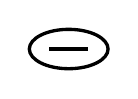
\begin{tikzpicture}[very thick]
          \draw (0,0) ellipse (0.5cm and 0.25cm);
          \draw (-0.25,0) -- (0.25,0);
        \end{tikzpicture}
      }
      ;
      \node[anchor=west] at (s4 -| 2,0) {Atributo llave};
      \node[anchor=north,inner sep=8pt] (s5) at (s4.south)
      {
        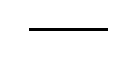
\begin{tikzpicture}[very thick] 
          \draw (-0.5,0) -- (0.5,0);
        \end{tikzpicture}
      }
      ;
      \node[anchor=west] at (s5 -| 2,0) {Conector};
      \node[anchor=east] at (\linewidth-30pt,-2) {  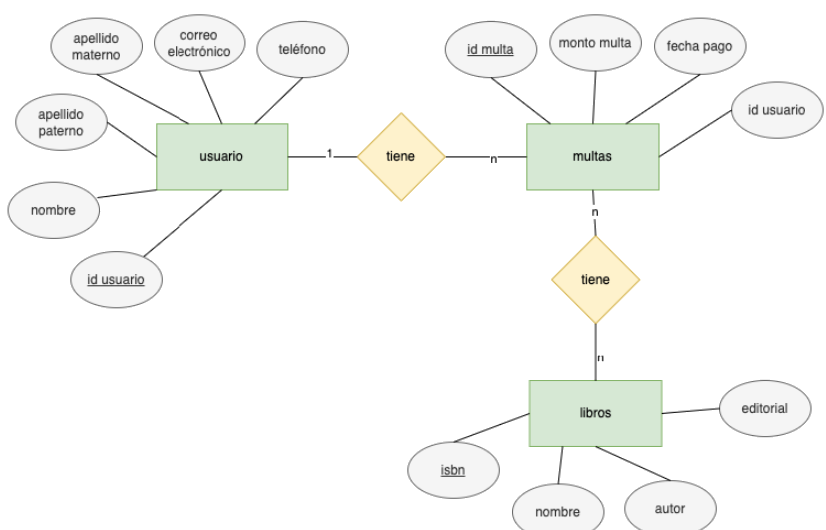
\includegraphics[height=4cm]{diagram.png}
      }
      ;

  \end{tikzpicture}

  \\
  Depenencias de existencia
  & Una entidad puede solo existir como "hijo" de otra
  \\
  Cardinalidad
  & \begin{minipage}{\linewidth}
    \# de registros de una entidad A que se relaciona con un registro de una entidad B

    \begin{itemize}
      \item 1-1: Un registro de A se relaciona únicamente con un registro de B 
      \item 1-n: Un registro de A se relaciona con 0 o varios registros de B 
      \item {n-n: Varios registros de A se relacionan con varios registros de B
          \medskip

          Se hace con una tabla adicional, solo con las relaciones
        }
    \end{itemize}
  \end{minipage}
  \\
  Primary Key / Clave primaria
  & {
    Número identificador del renglón en la tabla; único
    \medskip

    Se pueden usar para referenciar el renglón en otras tablas como clave foránea.
  }
  \\
  & {\Large\textbf{Normalización}}
  \\
  Significado y beneficios
  & \begin{minipage}{\linewidth}
    \begin{itemize}
      \item Elimina la redundancia: usa menos memoria
      \item Mejora la integridad de los datos: Si un dato se guarda dos veces, puede que no se actualice en un lugar y haya errores al buscar cosas en la tabla 
      \item Eliminación de anomalías: Sin la normalización puede ser necesario insertar valores incompletos (no inicializados, nulos, etc) 
      \item Eficiencia en la consulta y el manteniminento: Entre más grande y redundante la tabla, mas tardadas pueden ser las consultas y facilita hacer cambios a la base.
    \end{itemize}
  \end{minipage}
  \\
  1NF (1st normal form)
  & \begin{minipage}{\linewidth}
    \begin{itemize}
      \item Solo valores atómicos 
      \item No hay repticiones de grupos de datos o columnas que se puedan agrupar en una tabla separada 
      \item Cada fila es única y se puede identificar con una clave primaria
    \end{itemize}
    \medskip

    (Varias columnas para clases $\to$ una columna para clase y varios renglones con los mismos registros de alumno y una clase distinta por cada uno)
  \end{minipage}
  \\
  2NF
  & \begin{minipage}{\linewidth}
    \begin{itemize}
      \item cumple con 1nf 
      \item todos los campos no clave dependen completamente de la clave primaria
    \end{itemize}
    \medskip

    One (student\_id, name) and one (student\_id, class) table; no more redundance.
  \end{minipage}
  \\
  3NF
  & \begin{minipage}{\linewidth}
    \begin{itemize}
      \item cumple con 2NF
      \item No hay dependencias transitivas; Un atributo no clave no depende de otro atributo no clave
    \end{itemize}
    \medskip

    one (student\_id, name) and one (student\_id, class) table; no more redundance.
  \end{minipage}
  \\
  Dependencia transitiva
  & {
    Dadas las dependencias $A \to B$ y $B \to C$, entonces existe la dependencia transitiva de $C$ con respecto a $A$ si la dependencia $A \to B$ no existe directamente. En términos práctcos, $A$ sería una clave primaria, $B$ un atributo no clave y $C$ otro atributo no clave el cual depende de $B$.
    \medskip

    (student\_id, class\_id, class\_name) $\to$ (student\_id, class\_id) \& (class\_id, class\_name)
  }
  \\
  & {\Large\textbf{Modelo Lógico}}
  \\
  Objetivo
  & {
    Representar la información de manera logica con tablas, relaciones y restricciónes
  }
  \\
  Modelo Relacional
  & {
    Modelo para gestionar bases de datos propuesto por Edgar F. Codd. en 1970
    \medskip
  }
  \\
  Estructura
  & {
    Los datos dentro de las tablas se almacenan registros (filas), los cuales representan un objeto real, cada uno con varios atributos (columnas, campos).
    \medskip

    Cada fila se debe identificar con una \textbf{llave primaria} única.
    \medskip

    Las relaciones se establecen con llaves foráneas, columnas con las llaves primarias de otra tabla.
    \medskip

    Las relaciones pueden tener cardinalidad
  }
  \\
  Propiedades de las Tablas
  & {
    Cada tabla tiene un nombre y éste es distinto del nombre de todas las demás.
		\medskip

    Los valores de los campos son atómicos: encada registro, cada campo toma un solo valor.
		\medskip

    No hay dos camposen la misma tabla que se llamen igual.
		\medskip

    El orden de los campos no importa.
		\medskip

    Cada registroes distinta a las demás.
		\medskip

    El orden de los registros no importa.
  }
  \\
  NULL
  & La ausencia de un valor
  \\
  & {\Large\textbf{Integridad de datos}}
  \\
  & \begin{minipage}{\linewidth}
    \begin{itemize}
      \item Evita la duplicidad 
      \item Impide almacenar datos incorrectos 
      \item Impide altración de datos 
      \item Impide la eliminación de información
    \end{itemize}
  \end{minipage}

  \\
  Reglas de integridad de datos
  & \begin{minipage}{\linewidth}
    \begin{enumerate}
      \item Restricción de dominios (tipos de dato) 
      \item Regla de integridad de entidades: Ninguna llave primaria puede ser nula 
      \item Regla de integridad referencial: Cant make a referenced key null?
    \end{enumerate}
  \end{minipage}
  \\
  Reglas de nulos
  & \begin{minipage}{\linewidth}
    \begin{enumerate}
      \item Ningún campo de llave externa puede ser nulo
      \item Regla de integridad de entidades: Ninguna llave primaria puede ser nula 
      \item Regla de integridad referencial: Cant make a referenced key null?
    \end{enumerate}
  \end{minipage}
  \\
  Reglas de llaves externas: Borrado
  & \begin{minipage}{\linewidth}
    \begin{enumerate}
      \item Restringir: No se permite borrar el registro de la tabla dominante (\# 1) si existe un registro en una tabla subordinada (\#n)
      \item Propagar: El eliminar la dominante, el DBMS borra la subordinada
      \item Anular: El eliminar la dominante, convierte las referencias en la tabla subordinada a NULL
    \end{enumerate}
  \end{minipage}
  \\
  Reglas de llaves externas: Modificación
  & \begin{minipage}{\linewidth}
    \begin{enumerate}
      \item Restringir: Lo mismo cambiando eliniar por modificar
      \item Propagar: 
      \item Anular:
    \end{enumerate}
  \end{minipage}
  \\
  & MISSING SYMBOLOGY
  \\
  Reglas de negocio
  & {Restriciones espefíficas, dependientes del uso en la vida real, que se imponen a los datos
  }
  \\
  & {\Large\textbf{Álgebra relacional}}
  \\
  Definición
  & Un conjunto de operaciones que se aplican a relaciones (tablas) para producir nuevas tablas como resultados.
  \\
  Operaciones de conjuntos
  & \begin{minipage}{\linewidth}
    \begin{itemize}
      \item Unión
      \item Intersección 
      \item Diferencia
    \end{itemize}
  \end{minipage}
  \\
  Operaciones que remueven parte de una tabla
  & \begin{minipage}{\linewidth}
    \begin{itemize}
      \item Proyección: Table $\to$ new table with only some columns
      \item Selección: Table $\to$ new table with only some rows
    \end{itemize}
  \end{minipage}
  \\
  Producto carteseano
  & \begin{minipage}{\linewidth}
    $\left\{(r,s) \forall r \in R, s \in S\right\}$
    \medskip

    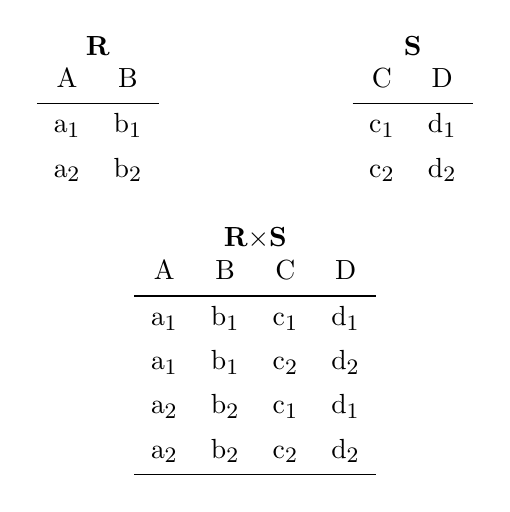
\begin{tikzpicture}
      \node[align=center] (R) at (0,0) {\textbf R\\

          \begin{tblr}{
            colspec={c c},
          }
            A & B \\
            \hline
            $a_1$ & $b_1$ \\
            $a_2$ & $b_2$ \\
          \end{tblr}
        };
      \node[align=center] (S) at (4,0) {\textbf S\\

          \begin{tblr}{
            colspec={c c},
          }
            C & D \\
            \hline
            $c_1$ & $d_1$ \\
            $c_2$ & $d_2$ \\
          \end{tblr}
        };
      \node[align=center] (RxS) at (2,-3) {\textbf R$\times$\textbf S\\

          \begin{tblr}{
            colspec={c c c c},
          }
            A & B &C & D \\
            \hline
            $a_1$ & $b_1$ & $c_1$ & $d_1$\\
            $a_1$ & $b_1$ & $c_2$ & $d_2$\\
            $a_2$ & $b_2$ & $c_1$ & $d_1$\\
            $a_2$ & $b_2$ & $c_2$ & $d_2$\\
            \hline
          \end{tblr}
        };
    \end{tikzpicture}
  \end{minipage}
  \\
  Natrual join
  & Producto cartesiano pero solo con los renglones que cumplan con cierta comparación "==" entre dos columnas
  \\
  Theta join
  & Lo mismo pero con mayor, menor, etc.
\end{longtblr}





\end{document}


